\subsection{粒子の回転が系に及ぼす影響}
粒子が系に存在することで生じる応力は,式\eqref{eq:system_stresslet}のように,
それぞれの粒子が存在することによる応力の総和を系の体積で割ることで求めることができる\cite{dilute_squirmer}.

    \begin{equation}
        \boldsymbol{\Sigma}^\mathrm{(p)} = \frac{1}{V} \sum \boldsymbol{S}
        \label{eq:system_stresslet}
    \end{equation}

\noindent
系に存在する粒子が,squirmer単体である場合には,その存在による応力は,式\eqref{eq:solitary_squirmer_stresslet}のように表される\cite{dilute_squirmer}.

    \begin{equation}
        \boldsymbol{S}_\mathrm{sol} = \frac{4}{3} \pi a^2 (3 \boldsymbol{ee} - \boldsymbol{I}) B_2
        \label{eq:solitary_squirmer_stresslet}
    \end{equation}

\noindent
式\eqref{eq:solitary_squirmer_stresslet}を\eqref{eq:system_stresslet}に代入し,
squirmerの方向ベクトルを成分表示し,応力の$xy$成分を抽出すると,式\eqref{eq:stresslet_xy}のように表される.

    \begin{align}
        \Sigma^\mathrm{(p)}_{xy} &= \frac{4 \pi a^2 B_2}{V} e_x e_y \notag \\
            &= \frac{4 \pi a^2 B_2}{V} \sin \theta \cos \theta
        \label{eq:stresslet_xy}
    \end{align}

\noindent
この応力は,$B_2 > 0$の場合,Fig.\ref{fig:stresslet_xy}のように表される.

    \begin{figure}[H]
        \centering
        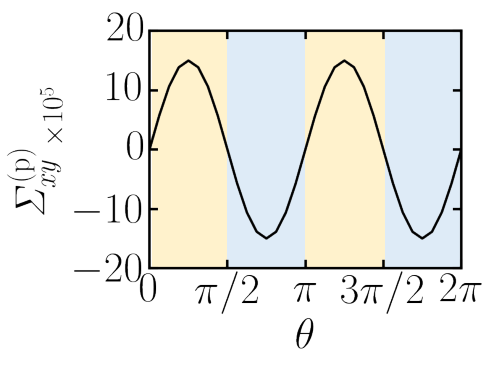
\includegraphics[scale=0.8]{/Users/taiga/Projects/lab/thesis/components/chapter3/figs/bottom_heavy_torque.pdf}
        \caption{単体squirmerの存在による応力の$xy$成分}
        \label{fig:stresslet_xy}
    \end{figure}

\noindent
このグラフより,粒子が定常的に回転している場合には,粒子の存在による応力の時間平均をとると,
プラスとマイナスで打ち消し合い,系に影響は与えないと予想される.
一方,粒子の進行方向がオレンジ色で示した範囲内に固定される場合には,
系の応力を大きくする方向にはたらき,
水色で示した範囲内に固定される場合には,
系の応力を小さくする方向にはたらくことが分かる.
$B_2<0$の場合は逆に,粒子の進行方向がオレンジ色で示した範囲内に固定される場合には,
系の応力を小さくする方向にはたらき,
水色で示した範囲内に固定される場合には,
系の応力を大きくする方向にはたらくことが分かる.
ここで,\ref{sec:purpose}で述べた有効粘度の式を再掲する.

    \begin{equation}
        \eta_\mathrm{eff} = \frac{\sigma}{\dot{\gamma}}
        \tag{\ref{eq:effective_viscosity}}
    \end{equation}

\noindent
この式から,系にはたらく応力が大きくなると有効粘度は大きくなり,応力が小さくなると有効粘度は小さくなることがわかる.
したがって,\ref{sec:rotation}で述べたように,squirmerの進行方向が,$0 \leq \theta < \pi /2$で固定された場合,
Puller型の場合は,有効粘度を大きくする方向にはたらき,Pusher型の場合は,有効粘度を小さく方向にはたらくことが予想される.
